\documentclass[a4paper,
               %boxit,
               %titlepage,   % separate title page
               %refpage      % separate references
              ]{jacow}

\ifboolexpr{bool{xetex} or bool{luatex}} % test for XeTeX/LuaTeX
 {}                                      % input encoding is utf8 by default
 {\usepackage[utf8]{inputenc}}           % switch to utf8

\usepackage{graphicx, subfigure}
\usepackage{booktabs}


\begin{document}
\title{BEAM COUPLING IMPEDANCE OF THE NEW BEAM SCREEN OF THE LHC INJECTION KICKER MAGNETS}
\author{H. Day\thanks{hugo.day@hep.manchester.ac.uk}, M.J. Barnes;  CERN, Switzerland}

\maketitle 


\begin{abstract}
The LHC injection kicker magnets (MKIs) experienced strong heating during the first operational run, identified as being caused by power loss due to wakefields induced by stored beam. Studies of the beam coupling impedance of the beam screen, a series of conductors embedded in a ceramic tube placed in the ferrite yoke to screen the ferrite from the beam, resulted in new design offering improved screening: this is predicted to reduce the heating to acceptable levels for operation with 25ns beam during run 2 of the LHC. However higher beam intensities proposed for HL-LHC operation are predicted to again cause strong heating to occur. Further studies have been carried out to reduce the beam induced power loss by optimising the beam screen design, some key results and findings of which are presented here.
\end{abstract}

\section{Introduction}

The injection kicker magnets (MKIs) are fast pulsed transmission line kicker magnets, which have a ceramic tube inserted into the ferrite yoke: this supports a number of screen conductors, designed to provide a good conducting path for the image currents of the circulating beam. One end of the screen is directly connected to the beam pipe whilst the other is capactively coupled to the beam pipe in order to preserve the fast field rise time of the magnet, shown in Fig.~\ref{fig:mkiStruct}. Beam-induced heating due to high stored beam current lead to high temperatures being observed in devices in the LHC, including the MKIs \cite{mki-heatingTemp}. In the MKI this lead to problems as the temperature of the ferrite yoke rises above it's Curie temperature necessitating 2-3 hours waiting time between fills. Substantial work has been done reduce the power deposited by reducing the beam coupling impedance of the device - a revised beam screen was implemented on all magnets during long shutdown 1 (LS1) which is predicted to reduce the power loss to a degree where excessive heating will not be a problem with nominal LHC beam parameters \cite{mkiImp2014}. 

The planned high luminousity upgrade of the LHC (called HL-LHC) will involve a doubling of the beam current in the LHC under current nominal parameters \cite{HLLHCPara} - this is predicted to lead to again a four fold increase in the power loss to all devices in the LHC unless counter-measures are taken. To this end further improvements to the beam screen have been studied in order to reduce the power loss into the magnet whilst continuing to ensure good high voltage (HV) performance during pulsing and good field quality for operation.

Building on this success a new design has been proposed to satisfy competing needs of low rates of electrical breakdown, during magnet pulsing, and a low beam coupling impedance to reduce the power lost into the structure by wakefields; in addition to meeting strict requirements for magnet operation for field rise time and flat top ripple \cite{mkiUpgrade}. 

\begin{figure}
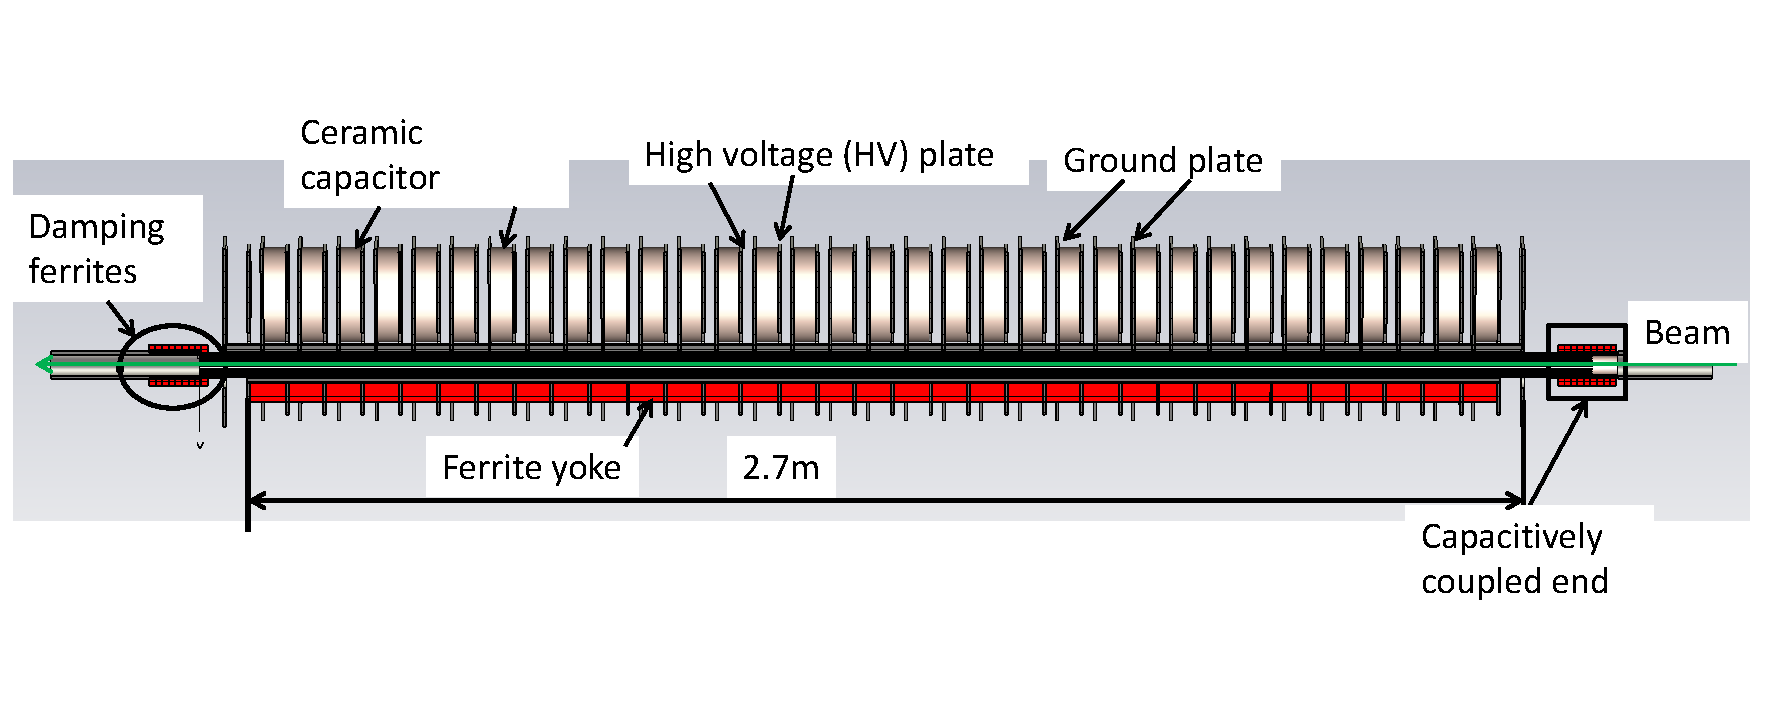
\includegraphics[width=0.5\textwidth]{MKICrossSectionYZ.pdf}
\caption{Structure of the injection kicker magnets.}
\label{fig:mkiStruct}
\end{figure}

\section{Changes to Beam Screen Design}

Past work on the beam screen of the MKI has focused on improving the screening of the ferrite yoke from the beam by increasing the number of screen conductors in the beam screen to the full compliment of 24 - during the first run of the LHC only 15 screen conductors were in place, positioned closest to the return busbar (see Fig.~\ref{fig:LengthWiseSlice}), due to issues with surface flashover during magnet pulsing \cite{mki-ElecBreakdown}. 

\begin{figure}
\begin{center}
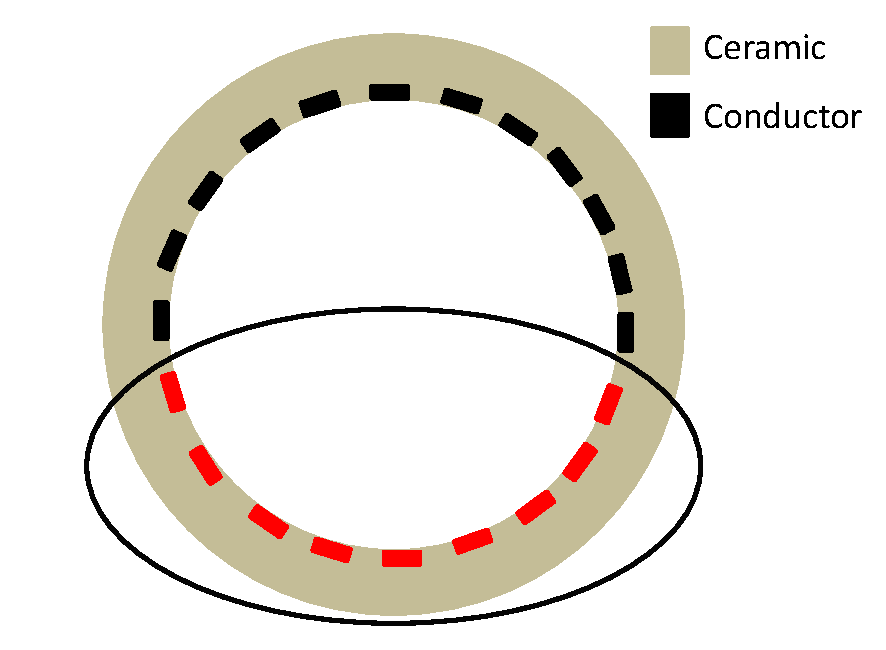
\includegraphics[width=0.25\textwidth]{sliceLabelled.pdf}
\caption{Cross-section of the beam screen of the MKI. Conductors circled in red weren't in place prior to long-shutdown 1}
\label{fig:LengthWiseSlice}
\end{center}
\end{figure}

A revised beam screen was designed that reduced the electric field strength during magnet pulsing sufficiently to allow 24 conductors to be inserted into the screen for post-LS1 \cite{mkiUpgrade}, shown in Fig.~\ref{fig:BeamScreenPostLS1}. This is predicted to see a substantial reduction in the power loss in the MKIs post LS1, by a factor of almost 2 (see Table~\ref{tab:PowLoss}), even accounting for the increased beam current with the change to 25ns bunch separation. However this is not expected to be sufficient for HL-LHC operation, which will see a much higher beam current than nominal LHC operation (see Table~\ref{tab:beamPara}) and is predicted to see power losses comparable to that which caused a faulty magnet to heat beyond it's point during early operation of the LHC \cite{mkiImp2014}, thus necessitating further modifications.

\begin{figure}
\begin{center}
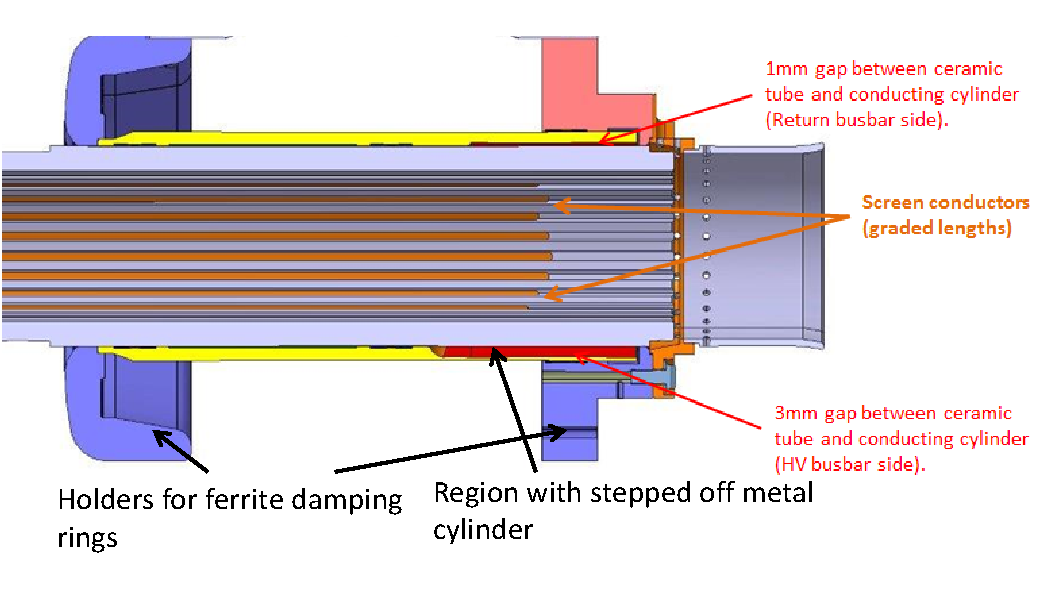
\includegraphics[width=0.5\textwidth]{beamScreenCrossSectionLabelled.pdf}
\caption{Cross-section of the beam screen of the MKI. Conductors circled in red weren't in place prior to long-shutdown 1}
\label{fig:BeamScreenPostLS1}
\end{center}
\end{figure}

\begin{table}
\caption{Power Loss for different beam screen arrangements with different beam parameters (see Tab.~\ref{tab:beamPara}) in W/m.}
\label{tab:PowLoss}
\begin{center}
\begin{tabular}{c | c | c}
Mode & 24 screen cond. & 15 screen cond. \\ \hline 
Pre-LS1 & 20-35 & 68 \\ \hline 
Post-LS1 & 34-52 & 117 \\ \hline 
HL-LHC, 50ns & 151-240 & 538  \\ \hline 
HL-LHC, 25ns & 125-191 & 432  \\ 
\end{tabular}
\end{center}
\end{table}

\begin{table}
\caption{Beam Parameters for different LHC operational modes}
\label{tab:beamPara}
\begin{center}
\begin{tabular}{c | c | c | c | c}
Mode & $\tau_{sep}$ (ns) & $N_{b}$ ($10^{11}$) & $ M $ & $t_{b}$ (ns) \\ \hline 
Pre-LS1 & 50 & 1.6 & $ 1380 $ & 1.2 \\ \hline 
Post-LS1 & 25 & 1.15 & 2808 & 1.0 \\ \hline 
HL-LHC, 50ns & 50 & 3.5 & 1380 & 1.0 \\ \hline 
HL-LHC, 25ns & 25 & 2.2 & 2808 & 1.0 \\ 
\end{tabular}
\end{center}
\end{table}

Previous work had showed that the beam coupling impedance the MKI with a well shielded ferrite yoke is resonant in nature, with the frequency of the resonances determined by the length of the overlap between the screen conductors on the internal face of the ceramic tube and the metal cylinder on the outside at the capacitively-coupled end of the tube, giving the form

\begin{equation}
f_{res} = \frac{nc}{2\sqrt{\epsilon_{r}}\left( L_{overlap}+ \delta_{fringe} \right)}
\end{equation}

where n is an integer, $\epsilon_{r}$ the relative permitivitty of the ceramic tube, $L_{overlap}$ the length of the overlap between the screen conductors and the external cylinder and $\delta_{fringe}$ the influence of the fringe fields on the effective length. For the post-LS1 design, $L_{overlap} = 117mm$. If we consider the general formula for power loss;

\begin{equation}
P_{loss} = 2 \left( f_{0} e M  N_{b}\right)^{2} \displaystyle\sum\limits_{n = -\infty}^{\infty}  \left| \lambda \left( p M \omega_{0} \right)  \right|^{2} \Re{}e \left[ Z_{\parallel} \left( p M \omega_{0} \right) \right]
\label{eqn:powLoss}
\end{equation}

where $f_{0}$ is the revolution frequnecy, $\omega_{0} = 2\pi f_{0}$, $e$ is the charge of an electron, $N_{b}$ is the number of particles per bunch, $M$ is the number of bunches in the machine, $\lambda (\omega)$ is the beam current spectrum, and $\Re{}e(Z_{\parallel}(\omega))$ is the real component of the longitudinal beam coupling impedance; we can see that we can reduce the power loss by changing the beam profile (in this case limited as the beam profile is determined by the requirements for the physics experiments) or the beam impedance profile may be modified. Due to the approximately gaussian roll off of the beam current spectrum at higher frequencies it can be seen that shortening $L_{pverlap}$ would result in the resonant frequency increasing. This approach was thus chosen due to the relative simplicity of the change (no major redesign of the magnet would be foreseen in this case) and the system being well proven for both HV and beam impedance factors.

In addition to the reduced overlap length, further alterations to the beam screen have been proposed for HV purposes in order to reduce the rate of surface flashover during magnet pulsing, shown in Fig.~\ref{fig:BeamScreenHLLHC}. These changes involve changes significant for the beam coupling impedance; a small air gap is introduced around the entire ceramic tube apart from a 90$^{\circ}$ arc at the top of the cylinder, being a maximum of 1mm at the bottom of the tube and tapering to 0mm. Due to the high permitivitty of the ceramic ($\epsilon_{r}\approx 10$) the small air gap greatly decreases the capacitance of the capactively coupled end, causing the frequency of a resonance for a fixed length of overlap to increase. 

\begin{figure}
\begin{center}
%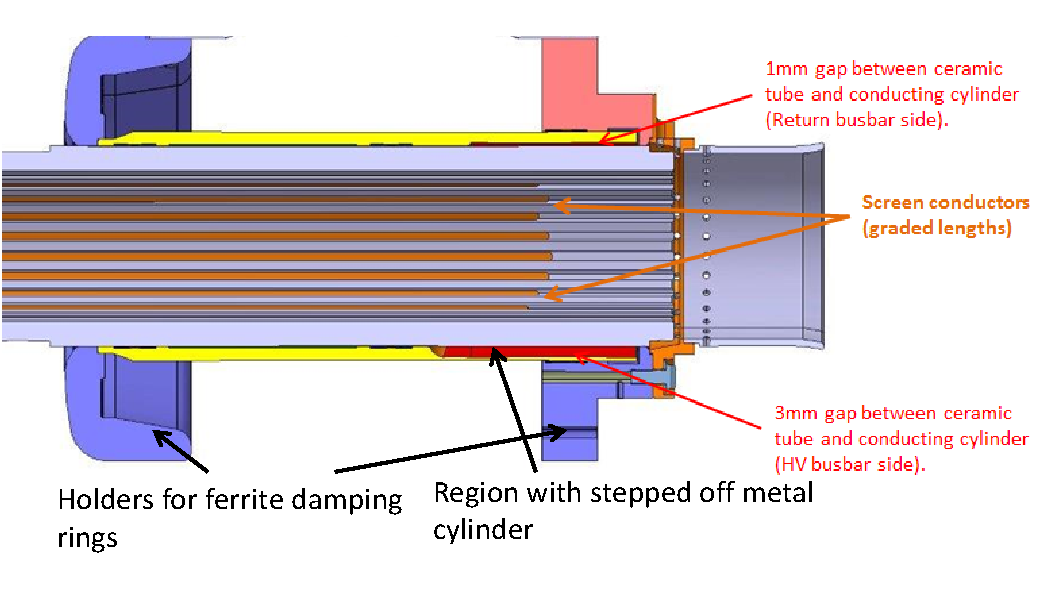
\includegraphics[width=0.5\textwidth]{beamScreenCrossSectionLabelled.pdf}
\caption{Cross-section of the proposed beam screen for the MKI under HL-LHC conditions.}
\label{fig:BeamScreenHLLHC}
\end{center}
\end{figure}

To illustrate this, simulations were carried out of the following cases, each with $L_{overlap}$=107mm: a) as the post-LS1 setup, b) a 1mm air-gap between the tube and the external cylinder, c) as for (b) but the air is replaced by ceramic, d) an offset air-gap, resulting in a gap of 1mm at the bottom and 0mm at the top using CST Particle Studio \cite{cst-cite}. The results are shown in Fig.~\ref{fig:differentEndArrangement} - it can be seen that the addition of the 1mm air-gap causes the resonant frequency to increase, moving to 610MHz for the fundamental frequency, compared to 461MHz for the standard screen design . It can be seen from the corresponding small shift in frequency from 1mm of ceramic that the shift is purely due to the permitivitty of the air, as the 1mm of ceramic gives a very small decrease, attributable to the increased thickness of ceramic leading to stronger influence of fringe fields. This offset air gap leads to an increase in the resonant frequency, but not as large as a uniform airgap - understandable as the capacitance does not decrease as much as a uniform gap.

\begin{figure}
\begin{center}
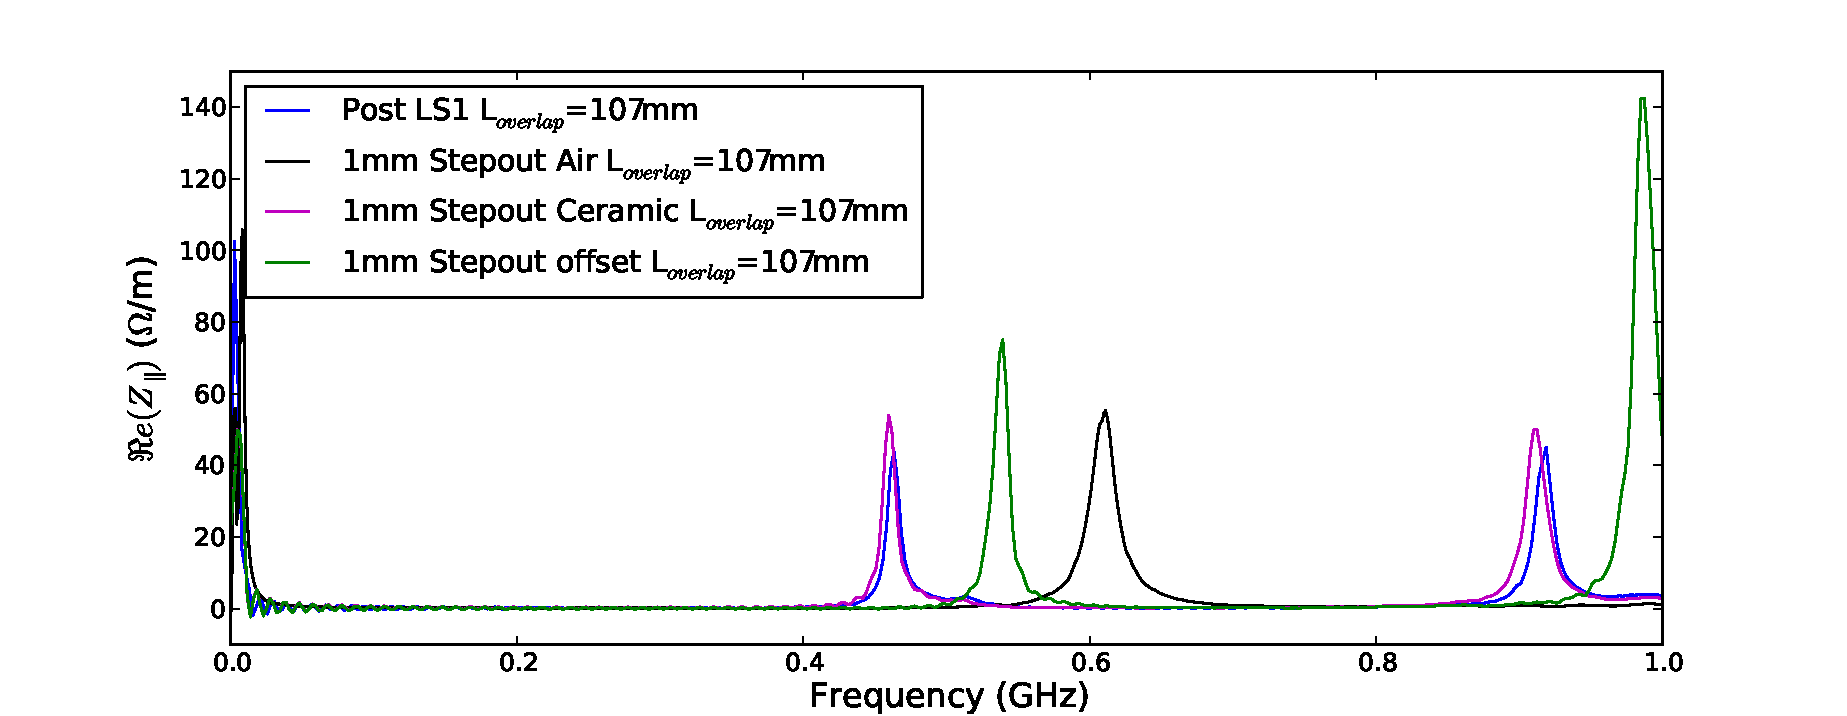
\includegraphics[width=0.5\textwidth]{differentScreenSpacings.pdf}
\caption{Real component of the longitudinal beam coupling impedance of an MKI with different beam screen arrangements}
\label{fig:differenEndArrangement}
\end{center}
\end{figure}

\section{Change in Overlap Length}

Initial investigations of the optimum overlap length were carried out using a reduced simulation of the MKI beam screen (only considering the capacitively coupled end of the beam screen, and simulating up to 1.1GHz) - the resulting power loss (N.B. not comparable to the results given previously as the magnitude of the resonances will be incorrect and the whole frequency range is not covered, but the frequencies will be comparable) is given in Fig.~\ref{fig:powLossLowRes}, covering lengths of 60,70,80,90,100,110 and 160mm. It can be seen that shortening the screen conductors to be less than 80mm in length could give substantial reductions in power loss.

\begin{figure}
\begin{center}
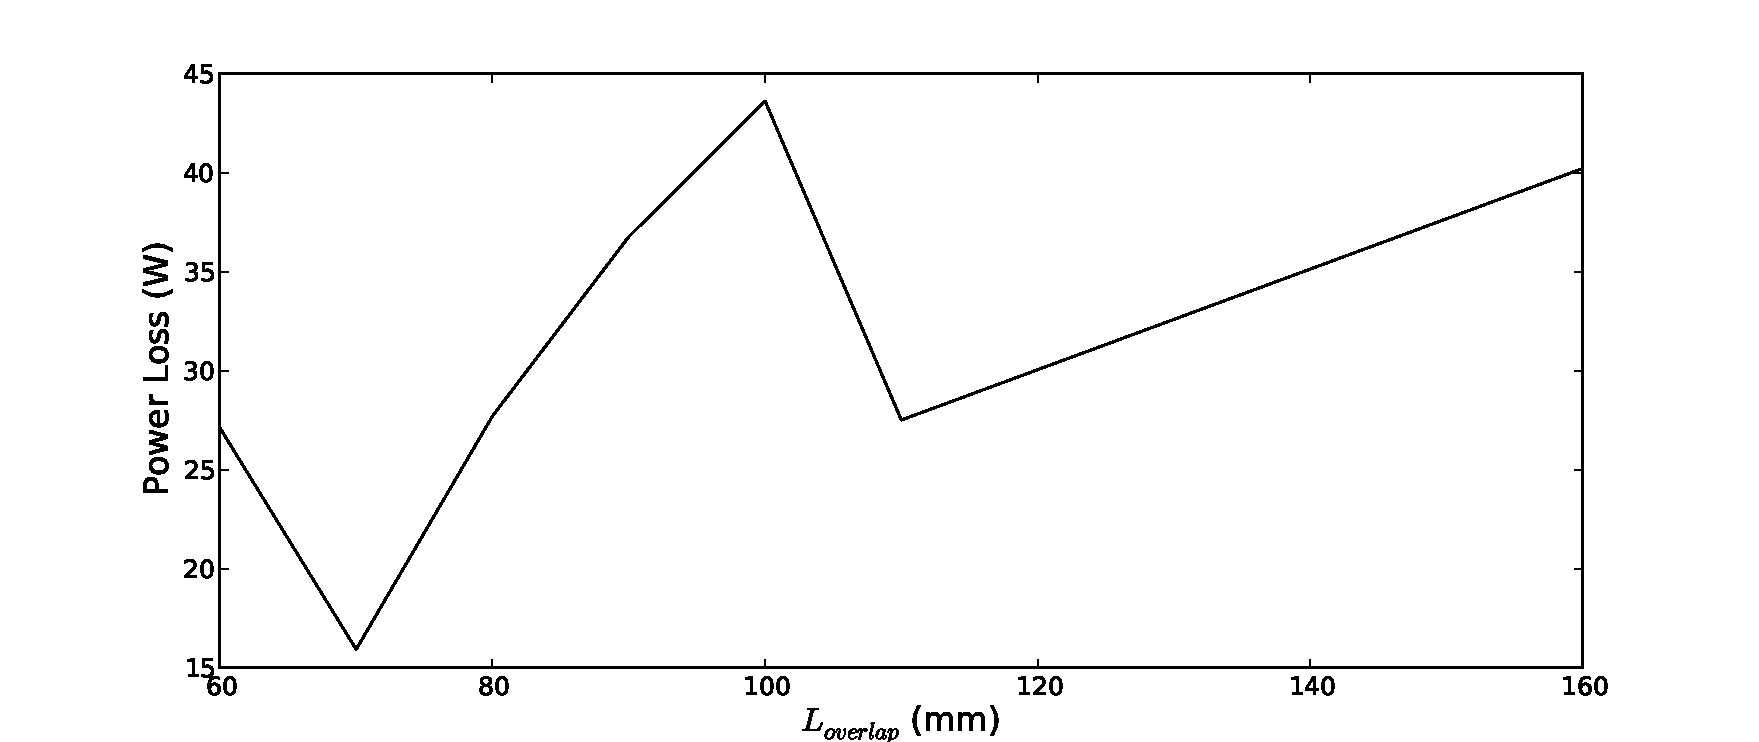
\includegraphics[width=0.5\textwidth]{powLossLowRes.pdf}
\caption{Power loss calculated from simulations of a reduced model of the MKI beam screen with different lengths of overlap between conductors and external cylinder}
\label{fig:powLossLowRes}
\end{center}
\end{figure}

On this basis a number of overlap lengths were simulated with a full model of the HL-LHC type design and coveriing the full frequency range, in addition to being manufactured for measurements within an MKI magne - this serves to verify the simulation data against measurements, important due to the relatively small frequency resolution of the measurements due to : $L_{overlap}$ = 59, 69, 79, 89, 99 and 119mm. 

Measurements are carried out using two methods; the resonant coxial wire method \cite{DayThesis}, used as it gives very accurate measurements of the beam coupling impedance, although with poor frequency resolutionm as the impedance of the MKI with a complete beam screen is expected to be very low, and using the classical transmission method, but without matching resistors and using time domain gating, used as although the magnitude of the impedance measured will not represent the true impedance, the frequency resolution is better than for the resonant method and it allows the measurements to be done quickly, which making resistive matching for each does not. This second method also guarantees that no resonances are missed by the resonant method - possible due to it's poor frequency resolution.

The results of the simulations and measurements with time-domain gating are shown in Fig.~\ref{fig:simMeasComp}; the solid lines are the measurements with gating and the dashed lines the simulation results. It can be seen that the resonant frequency increases in simulations and measurements as the overlap length is decreased, as expected. There is a difference in the resonant frequnecie given by the simulations and measurements; this is attributable to simulating the full model - in this case the small air gap (~1mm at most) at the capacitively coupled end of the beam screen is liable to generate errors in meshing in some cases causing the model the assume a metal on the surface of the ceramic as opposed to an air gap.

\begin{figure}
\begin{center}
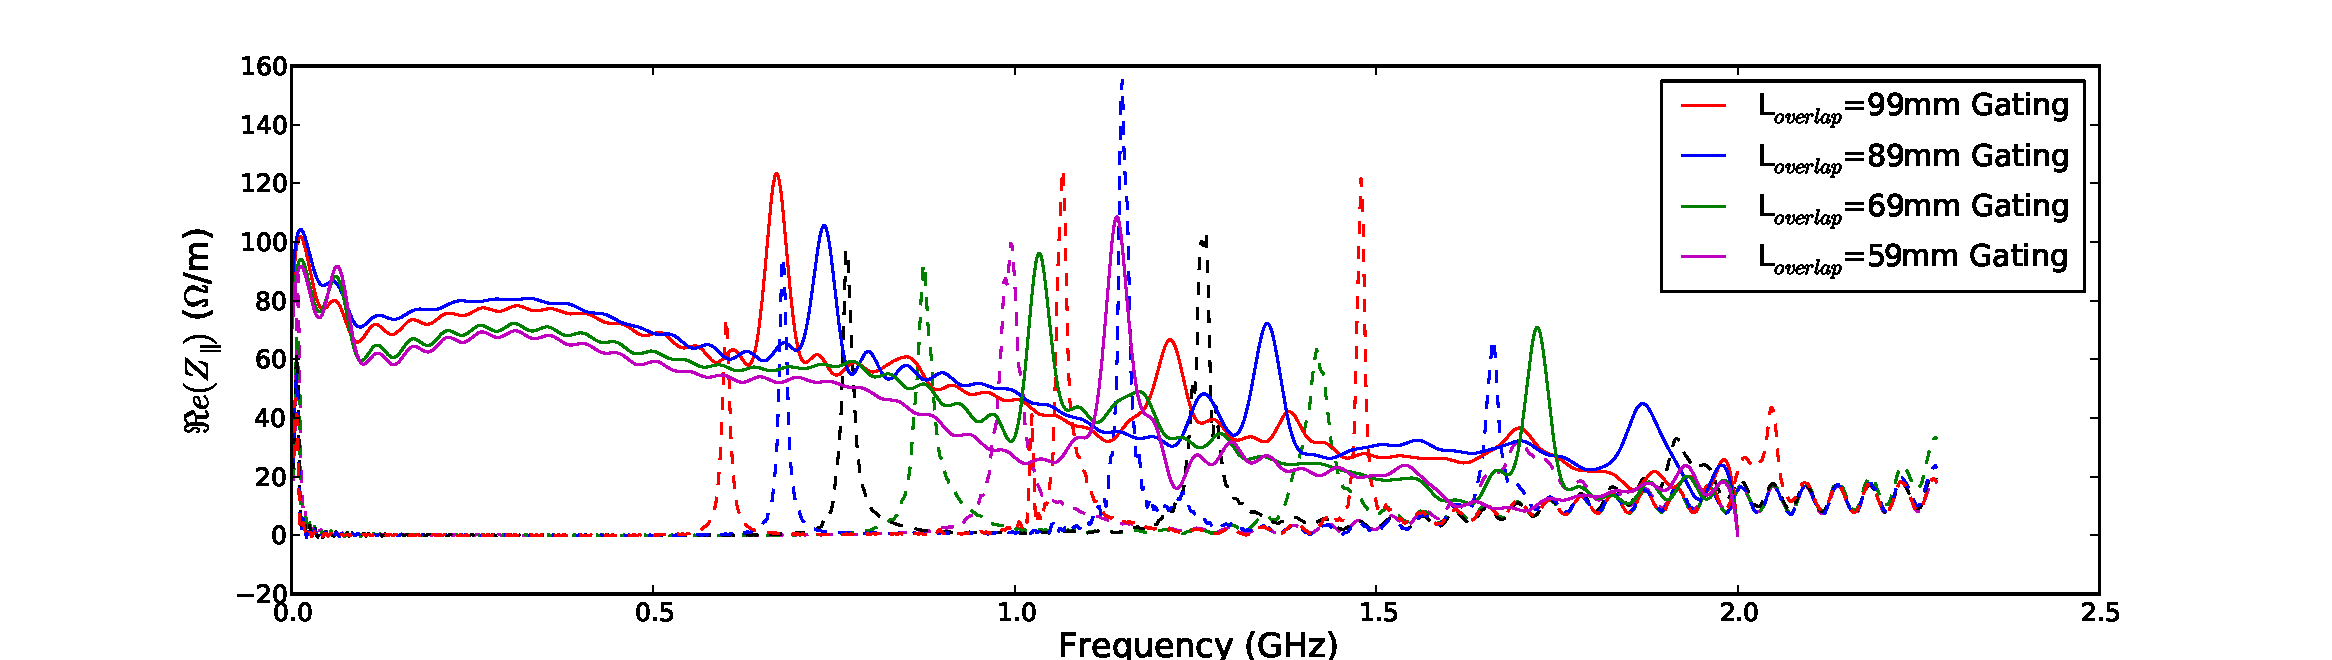
\includegraphics[width=0.5\textwidth]{simMeasGatingOverlap.pdf}
\caption{Comparison of the real component of the longitudinal beam coupling impedance between simulations and measurements of different overlap lengths}
\label{fig:simMeasComp}
\end{center}
\end{figure}

The power lost per metre is shown in Fig.~\ref{fig:powLossTotal} for measurements made using the resonant wire method, calculated using Eqn.~\ref{eqn:powLoss} and nominal 25ns LHC parameters. It can be seen that the a length less than 80mm gives a substantial ($\approx$20\%) reduction in power loss over lengths in the 110-120mm range, 38W/m compared to 47W/m. This indicates that a value of $L_{overlap}$ between 70-80mm would be optimum minimising the power loss.

\begin{figure}
\begin{center}
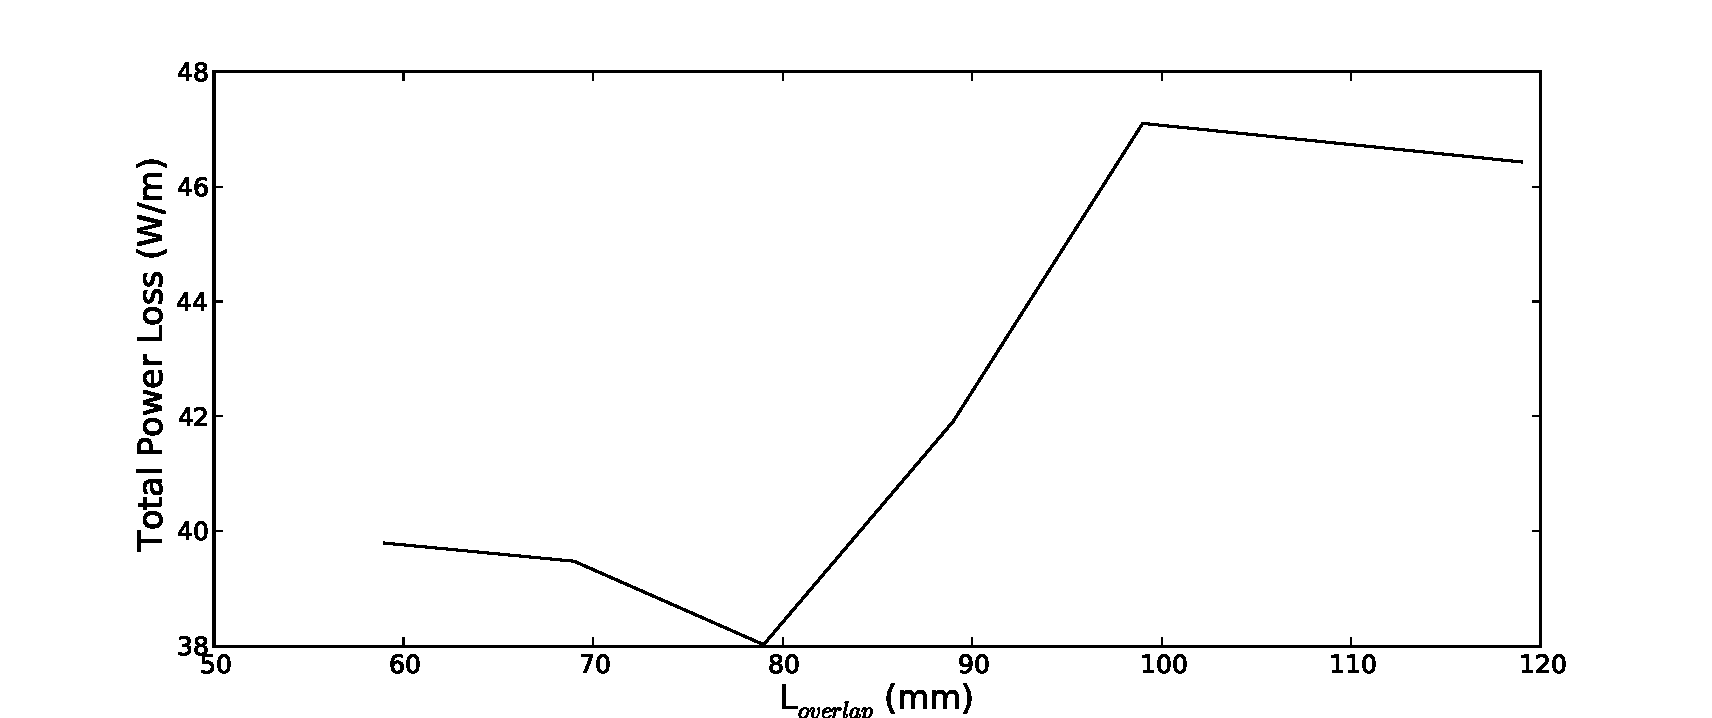
\includegraphics[width=0.5\textwidth]{heatingOverlapFull.pdf}
\caption{Power lost per metre for a number of overlap lengths, calculated assuming nominal LHC parameters using resonant wire measurements}
\label{fig:powLossTotal}
\end{center}
\end{figure}


\section{Summary and further work}

Further work to improve the impedance of the beam screen of the LHC injection kicker magnets has been carried out with a view to guarantee beam-induced heating doesn't become a problem during HL-LHC operation. It's been proposed to reduce the overlap at the capacitively coupled end to less than 80mm, preferring a value of $\approx$70mm. Further work remains to be done on verifying the design for HV behaviour and it is foreseen to place a prototype MKI with this and other modifications (particularly improvements to the cooling of the ferrite yoke) in either the LHC or SPS to verify the changes under operational conditions.


\begin{thebibliography}{9}

\bibitem{HLLHCPara}
O. Brüning, F. Zimmermann, \emph{"Parameter Space for the LHC High-Luminosity Upgrade"}, CERN-ATS-2012-070 

\bibitem{mki-heatingTemp}
M.J. Barnes \emph{et al}., \emph{"Beam Induced Ferrite Heating of the LHC Injection Kickers and Proposals for Improved Cooling"}, IPAC'13, Shanghai, China, MOPWA031.

\bibitem{mkiUpgrade}
M.J. Barnes \emph{et al}., \emph{Upgrade of the LHC Injection Kicker Magnets}, IPAC'13, Shanghai, China, MOPWA030

\bibitem{mki-ElecBreakdown}
M.J. Barnes \emph{et al}., \emph{"Reduction of Surface Flashover of the Beam Screen of the LHC Injection Kickers"}, IPAC'13, Shanghai, China, MOPWA031.

\bibitem{DayThesis}
PhD Thesis, H. Day, 2013.

\bibitem{mkiCoolling}
M. Barnes \emph{et al}., \emph{"Cooling of the LHC Injection Kicker Magnet Ferrite Yoke: Measurements and Future Proposals"}, IPAC'14, Dresden, Germany, MOPME075.

\bibitem{mkiImp2014}
H. Day \emph{et al}., \emph{"Beam Coupling Impedance of the New Beam Screen of the LHC Injection Kicker Magnets"}, IPAC'14, Dresden, Germany, TUPRI030.
\bibitem{cst-cite}
\texttt{http://www.cst.com}.

\end{thebibliography}
\end{document}

